\documentclass{beamer}

% Theme selection - auto-detect UASLP1 or fallback to Madrid
\IfFileExists{beamerthemeUASLP1.sty}{
    \usetheme{UASLP1}
}{
    \usetheme{Madrid}
    \usecolortheme{seahorse}
}

% Packages
\usepackage[utf8]{inputenc}
\usepackage[T1]{fontenc}
\usepackage{lmodern}
\usepackage{tikz}
\usepackage{listings}
\usepackage{xcolor}
\usepackage{amsmath}
\usepackage{hyperref}

% TikZ libraries
\usetikzlibrary{shapes.geometric, arrows.meta, positioning, fit, backgrounds}

% Code listing style
\lstset{
    language=C,
    basicstyle=\ttfamily\small,
    keywordstyle=\color{blue}\bfseries,
    commentstyle=\color{green!60!black}\itshape,
    stringstyle=\color{red},
    showstringspaces=false,
    breaklines=true,
    frame=single,
    numbers=left,
    numberstyle=\tiny\color{gray},
    tabsize=2,
    captionpos=b
}

% Title information
\title[USP Course 4: Multiprotocol]{Course 4: Multiprotocol Development}
\subtitle{USP Training Series}
\author{USP Development Team}
\institute{Universal Software Platform}
\date{\today}

\begin{document}

% Title slide
\begin{frame}
\titlepage
\end{frame}

% Table of contents
\begin{frame}{Course Overview}
\tableofcontents
\end{frame}

% ============================================================================
\section{Introduction}
% ============================================================================

\begin{frame}{Course 4: Multiprotocol Development}
\begin{block}{Learning Objectives}
\begin{itemize}
    \item Implement ping-pong bidirectional communication
    \item Measure and analyze Packet Error Rate (PER)
    \item Use LoRa ranging for distance measurement
    \item Develop multiprotocol applications with RAC
    \item Integrate custom protocols with LoRaWAN
\end{itemize}
\end{block}

\vspace{0.5cm}

\begin{block}{Hands-On Labs}
\begin{itemize}
    \item Lab 4.1: Ping-Pong Communication
    \item Lab 4.2: PER Testing
    \item Lab 4.3: LoRa Ranging
    \item Lab 4.4: Multiprotocol Application
\end{itemize}
\end{block}
\end{frame}

\begin{frame}{Prerequisites}
\begin{itemize}
    \item Completion of Course 3 (USP \& RAC Architecture)
    \item Understanding of RAC transaction model
    \item Familiarity with LR1120/LR1121 radio operations
    \item Knowledge of LoRa modulation parameters
    \item Two development boards for bidirectional testing
\end{itemize}

\vspace{0.5cm}

\begin{alertblock}{Hardware Requirements}
Two Xiao nRF54L15 + LR1120 boards required for Labs 4.1-4.3
\end{alertblock}
\end{frame}

% ============================================================================
\section{Ping-Pong Communication}
% ============================================================================

\begin{frame}{Ping-Pong Communication Overview}
\begin{columns}
\column{0.5\textwidth}
\begin{block}{What is Ping-Pong?}
Bidirectional LoRa communication where two devices alternately transmit and receive messages.
\end{block}

\vspace{0.3cm}

\textbf{Use Cases:}
\begin{itemize}
    \item Range testing
    \item Link quality assessment
    \item Protocol development
    \item Bidirectional data exchange
\end{itemize}

\column{0.5\textwidth}
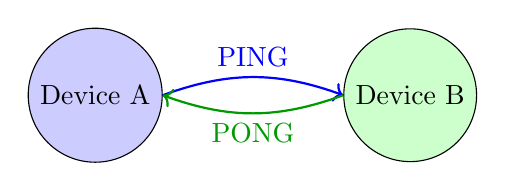
\begin{tikzpicture}[scale=0.8]
    % Device A
    \node[draw, circle, minimum size=1.5cm, fill=blue!20] (a) at (0,2) {Device A};
    \node[draw, circle, minimum size=1.5cm, fill=green!20] (b) at (5,2) {Device B};

    % Ping arrow
    \draw[->, thick, blue] (a.east) to[bend left=20] node[above] {PING} (b.west);

    % Pong arrow
    \draw[->, thick, green!60!black] (b.west) to[bend left=20] node[below] {PONG} (a.east);
\end{tikzpicture}
\end{columns}
\end{frame}

\begin{frame}[fragile]{Ping-Pong State Machine}
\begin{center}
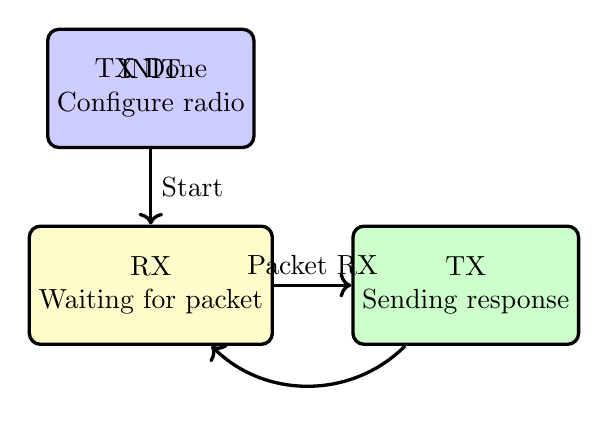
\begin{tikzpicture}[node distance=2.5cm, auto,
    state/.style={rectangle, rounded corners, draw=black, very thick, minimum height=1.5cm, minimum width=2cm, align=center}]

    \node[state, fill=blue!20] (init) {INIT\\Configure radio};
    \node[state, fill=yellow!20, below of=init] (rx) {RX\\Waiting for packet};
    \node[state, fill=green!20, right of=rx, node distance=4cm] (tx) {TX\\Sending response};

    \draw[->, very thick] (init) -- (rx) node[midway, right] {Start};
    \draw[->, very thick] (rx) -- (tx) node[midway, above] {Packet RX};
    \draw[->, very thick] (tx) to[bend left=45] (rx) node[midway, above] {TX Done};
\end{tikzpicture}
\end{center}

\vspace{0.3cm}

\textbf{Key Parameters:}
\begin{itemize}
    \item Timeout for RX mode (typically 5-10 seconds)
    \item TX/RX turnaround time
    \item Payload format (sequence number, RSSI, SNR)
\end{itemize}
\end{frame}

\begin{frame}[fragile]{Ping-Pong Implementation}
\begin{lstlisting}[caption={Ping-Pong Main Loop}]
typedef enum {
    STATE_RX,
    STATE_TX,
} pingpong_state_t;

static pingpong_state_t state = STATE_RX;
static uint32_t ping_count = 0;

void pingpong_event_handler(void) {
    if (radio_event == RADIO_RX_DONE) {
        // Packet received - extract payload
        uint8_t payload[256];
        uint8_t size;
        lr11xx_radio_get_rx_buffer_status(&size, &offset);
        lr11xx_regmem_read_buffer8(payload, offset, size);

        ping_count = (payload[0] << 8) | payload[1];
        int16_t rssi = payload[2];
        int8_t snr = payload[3];

        printk("RX: count=%u, RSSI=%d, SNR=%d\n",
               ping_count, rssi, snr);

        state = STATE_TX;  // Reply with pong
    }
}
\end{lstlisting}
\end{frame}

\begin{frame}[fragile]{Ping-Pong TX Implementation}
\begin{lstlisting}[caption={Transmit Pong Response}]
void pingpong_send_response(void) {
    uint8_t payload[4];

    // Increment ping count
    ping_count++;

    // Build payload
    payload[0] = (ping_count >> 8) & 0xFF;
    payload[1] = ping_count & 0xFF;
    payload[2] = last_rssi;
    payload[3] = last_snr;

    // Send via RAC
    rac_params_t params = {
        .priority = 128,
        .pre_callback = pingpong_tx_pre,
        .post_callback = pingpong_tx_post,
        .context = payload,
    };

    rac_add(&params, &pingpong_handle);
}
\end{lstlisting}
\end{frame}

% ============================================================================
\section{PER Testing}
% ============================================================================

\begin{frame}{Packet Error Rate (PER) Testing}
\begin{block}{What is PER?}
PER measures the percentage of packets that fail to be received correctly.

\[
\text{PER} = \frac{\text{Packets Lost}}{\text{Packets Sent}} \times 100\%
\]
\end{block}

\vspace{0.3cm}

\textbf{Why Measure PER?}
\begin{itemize}
    \item Evaluate link quality under real conditions
    \item Determine maximum communication range
    \item Optimize modulation parameters (SF, BW, CR)
    \item Validate antenna performance
    \item Compare different environments (urban, rural, indoor)
\end{itemize}
\end{frame}

\begin{frame}{PER Test Setup}
\begin{columns}
\column{0.5\textwidth}
\textbf{Test Configuration:}
\begin{itemize}
    \item Fixed transmitter (TX)
    \item Mobile receiver (RX)
    \item Continuous transmission
    \item Sequence number in payload
    \item RSSI/SNR logging
\end{itemize}

\vspace{0.3cm}

\textbf{Typical Test:}
\begin{itemize}
    \item Send 1000 packets
    \item Increase distance
    \item Record lost packets
    \item Calculate PER
\end{itemize}

\column{0.5\textwidth}
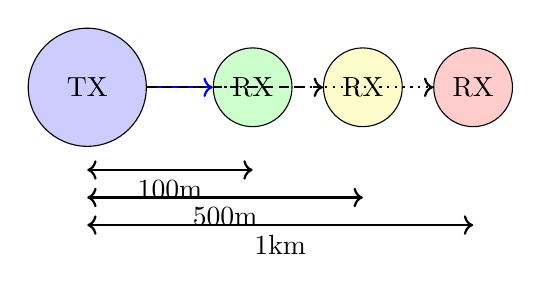
\begin{tikzpicture}[scale=0.7]
    % TX device
    \node[draw, circle, fill=blue!20, minimum size=1.5cm] (tx) at (0,0) {TX};

    % RX devices at different distances
    \node[draw, circle, fill=green!20, minimum size=1cm] (rx1) at (3,0) {RX};
    \node[draw, circle, fill=yellow!20, minimum size=1cm] (rx2) at (5,0) {RX};
    \node[draw, circle, fill=red!20, minimum size=1cm] (rx3) at (7,0) {RX};

    % Distance annotations
    \draw[<->, thick] (0,-1.5) -- (3,-1.5) node[midway, below] {100m};
    \draw[<->, thick] (0,-2) -- (5,-2) node[midway, below] {500m};
    \draw[<->, thick] (0,-2.5) -- (7,-2.5) node[midway, below] {1km};

    % Signal waves
    \draw[->, thick, blue] (tx) -- (rx1);
    \draw[->, thick, dashed] (tx) -- (rx2);
    \draw[->, thick, dotted] (tx) -- (rx3);
\end{tikzpicture}

\vspace{0.3cm}

\tiny
\begin{tabular}{|c|c|c|}
\hline
Distance & PER & Link \\
\hline
100m & 0.1\% & Excellent \\
500m & 2.5\% & Good \\
1km & 15\% & Poor \\
\hline
\end{tabular}
\end{columns}
\end{frame}

\begin{frame}[fragile]{PER Transmitter Implementation}
\begin{lstlisting}[caption={PER TX - Continuous Transmission}]
static uint32_t seq_number = 0;
static uint32_t total_packets = 0;

void per_tx_thread(void) {
    while (1) {
        // Build packet with sequence number
        uint8_t payload[8];
        payload[0] = (seq_number >> 24) & 0xFF;
        payload[1] = (seq_number >> 16) & 0xFF;
        payload[2] = (seq_number >> 8) & 0xFF;
        payload[3] = seq_number & 0xFF;
        payload[4] = 0xAA;  // Magic marker
        payload[5] = 0x55;

        // Transmit via RAC
        per_tx_packet(payload, sizeof(payload));

        seq_number++;
        total_packets++;

        // 1 second interval
        k_sleep(K_SECONDS(1));
    }
}
\end{lstlisting}
\end{frame}

\begin{frame}[fragile]{PER Receiver Implementation}
\begin{lstlisting}[caption={PER RX - Detect Lost Packets}]
static uint32_t last_seq = 0;
static uint32_t total_rx = 0;
static uint32_t total_lost = 0;

void per_rx_event_handler(void) {
    if (radio_event == RADIO_RX_DONE) {
        uint32_t seq = (payload[0] << 24) |
                       (payload[1] << 16) |
                       (payload[2] << 8) | payload[3];

        // Check for lost packets
        if (seq > last_seq + 1) {
            uint32_t lost = seq - last_seq - 1;
            total_lost += lost;
            printk("Lost %u packets!\n", lost);
        }

        last_seq = seq;
        total_rx++;

        float per = (float)total_lost /
                    (total_rx + total_lost) * 100.0f;
        printk("PER: %.2f%% (RX=%u, Lost=%u)\n",
               per, total_rx, total_lost);
    }
}
\end{lstlisting>
\end{frame}

\begin{frame}{PER Analysis and Interpretation}
\begin{block}{Link Budget Correlation}
PER results validate link budget calculations:
\begin{itemize}
    \item \textbf{PER < 1\%}: Excellent link, margin for fading
    \item \textbf{PER 1-5\%}: Good link, acceptable for most applications
    \item \textbf{PER 5-10\%}: Marginal link, retransmissions needed
    \item \textbf{PER > 10\%}: Poor link, move closer or increase SF
\end{itemize}
\end{block}

\vspace{0.3cm}

\textbf{Optimization Strategies:}
\begin{enumerate}
    \item Increase Spreading Factor (SF) $\rightarrow$ lower data rate, higher sensitivity
    \item Use lower bandwidth $\rightarrow$ better SNR
    \item Increase TX power $\rightarrow$ higher link budget
    \item Improve antenna positioning
    \item Enable Forward Error Correction (higher CR)
\end{enumerate}
\end{frame}

% ============================================================================
\section{LoRa Ranging}
% ============================================================================

\begin{frame}{LoRa Ranging Technology}
\begin{columns}
\column{0.6\textwidth}
\begin{block}{What is Ranging?}
LoRa ranging uses Time-of-Flight (ToF) measurements to determine the distance between two devices.
\end{block}

\vspace{0.3cm}

\textbf{How it Works:}
\begin{enumerate}
    \item Master sends ranging request
    \item Slave responds with ranging packet
    \item Radio measures round-trip time
    \item Distance calculated: $d = \frac{c \cdot t}{2}$
\end{enumerate}

\vspace{0.3cm}

\textbf{Accuracy:}
\begin{itemize}
    \item Typical: ±10-30m
    \item Best case: ±5m (open field)
    \item Worst case: ±50m (urban multipath)
\end{itemize}

\column{0.4\textwidth}
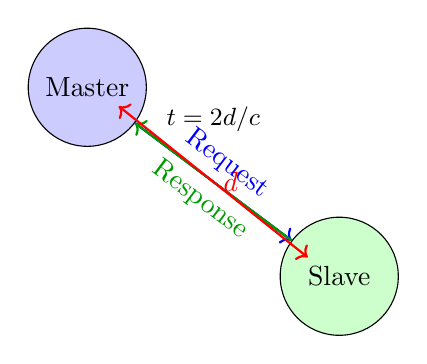
\begin{tikzpicture}[scale=0.8]
    % Master device
    \node[draw, circle, fill=blue!20, minimum size=1.5cm] (m) at (0,3) {Master};

    % Slave device
    \node[draw, circle, fill=green!20, minimum size=1.5cm] (s) at (4,0) {Slave};

    % Request arrow
    \draw[->, thick, blue] (m) -- (s) node[midway, above, rotate=-37] {Request};

    % Response arrow
    \draw[->, thick, green!60!black] (s) -- (m) node[midway, below, rotate=-37] {Response};

    % Distance annotation
    \draw[<->, thick, red] (0.5,2.7) -- (3.5,0.3) node[midway, right] {$d$};

    % Clock icon
    \node at (2,2.5) {\small $t = 2d/c$};
\end{tikzpicture}
\end{columns}
\end{frame}

\begin{frame}{Ranging Packet Exchange}
\begin{center}
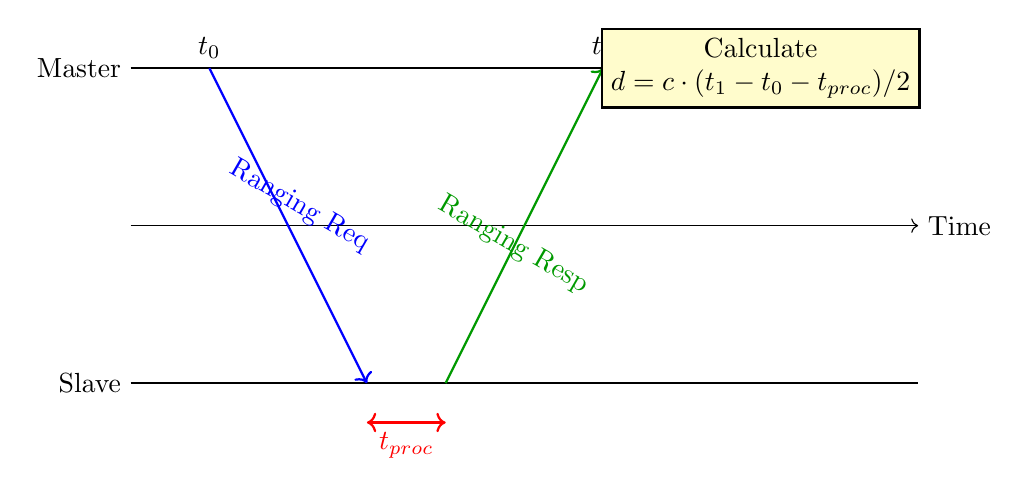
\begin{tikzpicture}[
    node distance=1.5cm,
    box/.style={rectangle, draw=black, thick, minimum height=1cm, minimum width=3cm, align=center}
]
    % Timeline
    \draw[->] (0,0) -- (10,0) node[right] {Time};

    % Master timeline
    \draw[thick] (0,2) -- (10,2);
    \node[left] at (0,2) {Master};

    % Slave timeline
    \draw[thick] (0,-2) -- (10,-2);
    \node[left] at (0,-2) {Slave};

    % Ranging request
    \draw[->, thick, blue] (1,2) -- (3,-2) node[midway, above, rotate=-30] {Ranging Req};
    \node[above] at (1,2) {$t_0$};

    % Processing delay
    \draw[<->, thick, red] (3,-2.5) -- (4,-2.5) node[midway, below] {$t_{proc}$};

    % Ranging response
    \draw[->, thick, green!60!black] (4,-2) -- (6,2) node[midway, below, rotate=-30] {Ranging Resp};
    \node[above] at (6,2) {$t_1$};

    % Distance calculation
    \node[box, fill=yellow!20] at (8,2) {Calculate\\$d = c \cdot (t_1 - t_0 - t_{proc})/2$};
\end{tikzpicture}
\end{center}

\vspace{0.3cm}

\textbf{Key Timing:}
\begin{itemize}
    \item $t_0$: Master sends request
    \item $t_{proc}$: Slave processing time (known, calibrated)
    \item $t_1$: Master receives response
    \item Distance: $d = \frac{c \cdot (t_1 - t_0 - t_{proc})}{2}$
\end{itemize}
\end{frame}

\begin{frame}[fragile]{Ranging Implementation - Master}
\begin{lstlisting}[caption={Initiate Ranging Request (Master)}]
void ranging_master_start(void) {
    // Configure ranging parameters
    lr11xx_radio_lora_ranging_params_t params = {
        .address = SLAVE_ADDRESS,
        .request_count = 10,  // Average 10 measurements
        .role = LR11XX_RADIO_LORA_RANGING_MASTER,
    };

    // Set ranging mode
    lr11xx_radio_set_lora_ranging(&params);

    // Start ranging transaction via RAC
    rac_params_t rac_params = {
        .priority = 200,
        .pre_callback = ranging_pre_callback,
        .post_callback = ranging_post_callback,
    };

    rac_add(&rac_params, &ranging_handle);
}
\end{lstlisting}
\end{frame}

\begin{frame}[fragile]{Ranging Implementation - Slave}
\begin{lstlisting}[caption={Respond to Ranging Request (Slave)}]
void ranging_slave_init(void) {
    // Configure as slave
    lr11xx_radio_lora_ranging_params_t params = {
        .address = MY_ADDRESS,
        .role = LR11XX_RADIO_LORA_RANGING_SLAVE,
    };

    lr11xx_radio_set_lora_ranging(&params);

    // Start continuous RX for ranging requests
    lr11xx_radio_set_rx(RX_CONTINUOUS);
}

void ranging_slave_event_handler(void) {
    if (radio_event == RADIO_RANGING_REQUEST_VALID) {
        // Radio automatically responds
        printk("Ranging request received\n");
    }
}
\end{lstlisting}
\end{frame}

\begin{frame}[fragile]{Extract Ranging Results}
\begin{lstlisting}[caption={Parse Ranging Results (Master)}]
void ranging_result_handler(void) {
    lr11xx_radio_lora_ranging_result_t result;

    lr11xx_radio_get_lora_ranging_result(&result);

    if (result.status ==
        LR11XX_RADIO_RANGING_STATUS_VALID) {

        float distance_m = result.distance_raw * 150.0f
                          / 4096.0f;  // Convert to meters

        int16_t rssi = result.rssi;

        printk("Distance: %.2f m, RSSI: %d dBm\n",
               distance_m, rssi);

        // Store for averaging
        store_ranging_sample(distance_m);
    }
}
\end{lstlisting>
\end{frame}

\begin{frame}{Ranging Applications}
\begin{columns}
\column{0.5\textwidth}
\textbf{Asset Tracking:}
\begin{itemize}
    \item Locate devices without GPS
    \item Indoor positioning
    \item Warehouse inventory
    \item Livestock tracking
\end{itemize}

\vspace{0.3cm}

\textbf{Proximity Detection:}
\begin{itemize}
    \item Social distancing
    \item Collision avoidance
    \item Access control
    \item Geofencing
\end{itemize}

\column{0.5\textwidth}
\textbf{Advantages over GPS:}
\begin{itemize}
    \item Works indoors
    \item Lower power consumption
    \item No satellite dependency
    \item Lower cost
\end{itemize}

\vspace{0.3cm}

\textbf{Limitations:}
\begin{itemize}
    \item Requires line-of-sight
    \item Affected by multipath
    \item Limited to LR11xx radios
    \item 2-device measurement only
\end{itemize}
\end{columns}
\end{frame}

% ============================================================================
\section{Multiprotocol Applications}
% ============================================================================

\begin{frame}{Multiprotocol Architecture with RAC}
\begin{center}
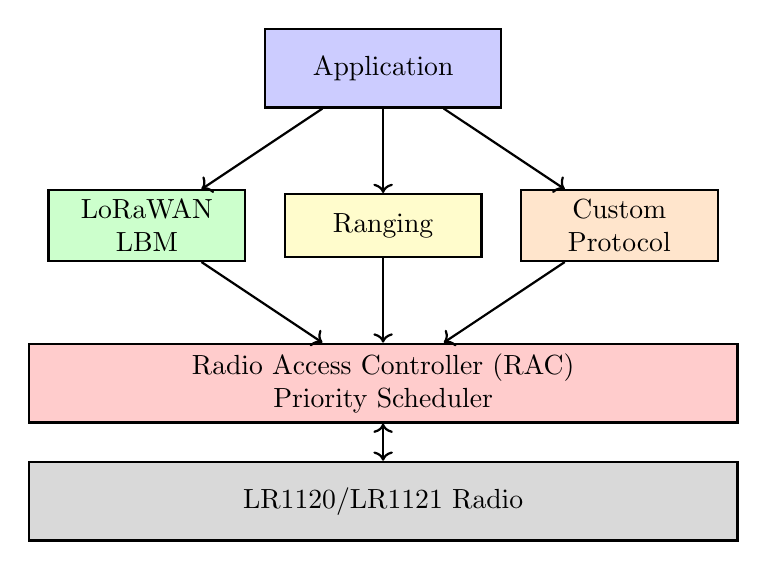
\begin{tikzpicture}[
    box/.style={rectangle, draw=black, thick, minimum height=1cm, minimum width=3cm, align=center, fill=blue!20},
    proto/.style={rectangle, draw=black, thick, minimum height=0.8cm, minimum width=2.5cm, align=center}
]
    % Application layer
    \node[box] (app) at (0,4) {Application};

    % Protocol handlers
    \node[proto, fill=green!20] (lorawan) at (-3,2) {LoRaWAN\\LBM};
    \node[proto, fill=yellow!20] (ranging) at (0,2) {Ranging};
    \node[proto, fill=orange!20] (custom) at (3,2) {Custom\\Protocol};

    % RAC layer
    \node[box, fill=red!20, minimum width=9cm] (rac) at (0,0) {Radio Access Controller (RAC)\\Priority Scheduler};

    % Radio hardware
    \node[box, fill=gray!30, minimum width=9cm] (radio) at (0,-1.5) {LR1120/LR1121 Radio};

    % Connections
    \draw[->, thick] (app) -- (lorawan);
    \draw[->, thick] (app) -- (ranging);
    \draw[->, thick] (app) -- (custom);

    \draw[->, thick] (lorawan) -- (rac);
    \draw[->, thick] (ranging) -- (rac);
    \draw[->, thick] (custom) -- (rac);

    \draw[<->, thick] (rac) -- (radio);
\end{tikzpicture}
\end{center}
\end{frame}

\begin{frame}{Multiprotocol Use Cases}
\begin{block}{LoRaWAN + Ranging}
Asset tracker that reports location via LoRaWAN and uses ranging for proximity detection.
\end{block}

\begin{block}{LoRaWAN + Custom Protocol}
Smart meter with LoRaWAN uplinks and local mesh networking for meter-to-meter communication.
\end{block}

\begin{block}{LoRaWAN + PER Testing}
Deployed sensor that performs periodic link quality tests while maintaining normal operation.
\end{block}

\vspace{0.3cm}

\textbf{Key Design Principles:}
\begin{itemize}
    \item Assign appropriate priorities (LoRaWAN highest)
    \item Respect duty cycle limits across all protocols
    \item Handle conflicts gracefully (RAC queuing)
    \item Use separate buffers for each protocol
\end{itemize}
\end{frame}

\begin{frame}[fragile]{Multiprotocol Priority Assignment}
\begin{lstlisting}[caption={Priority Configuration}]
// Priority levels (0 = highest, 255 = lowest)
#define PRIORITY_LORAWAN_EMERGENCY  0
#define PRIORITY_LORAWAN_CONFIRMED  50
#define PRIORITY_LORAWAN_UNCONFIRMED 100
#define PRIORITY_RANGING            150
#define PRIORITY_CUSTOM_PROTOCOL    200
#define PRIORITY_HEARTBEAT          250

void configure_protocols(void) {
    // LoRaWAN always has highest priority
    lbm_set_priority(PRIORITY_LORAWAN_CONFIRMED);

    // Ranging for asset tracking
    ranging_set_priority(PRIORITY_RANGING);

    // Custom protocol for local mesh
    custom_proto_set_priority(
        PRIORITY_CUSTOM_PROTOCOL);

    // Low-priority heartbeat
    heartbeat_set_priority(PRIORITY_HEARTBEAT);
}
\end{lstlisting}
\end{frame}

\begin{frame}[fragile]{Handle Protocol Conflicts}
\begin{lstlisting}[caption={Conflict Resolution}]
void ranging_request(void) {
    rac_params_t params = {
        .priority = PRIORITY_RANGING,
        .pre_callback = ranging_pre,
        .post_callback = ranging_post,
    };

    rac_status_t status = rac_add(&params, &handle);

    if (status == RAC_STATUS_BUSY) {
        // Higher priority TX in progress
        printk("Ranging deferred\n");

        // Retry later or queue request
        k_work_schedule(&ranging_retry_work,
                        K_SECONDS(5));
    } else if (status == RAC_STATUS_OK) {
        printk("Ranging started\n");
    }
}
\end{lstlisting}
\end{frame}

\begin{frame}{Duty Cycle Management}
\begin{block}{Challenge}
Multiple protocols must share limited duty cycle budget (typically 1\% in EU868).
\end{block}

\vspace{0.3cm}

\textbf{Solution Strategies:}
\begin{enumerate}
    \item \textbf{Global Budget:} Track total airtime across all protocols
    \item \textbf{Per-Protocol Limits:} Allocate budget to each protocol
    \item \textbf{Dynamic Allocation:} Unused budget can be borrowed
    \item \textbf{Adaptive Scheduling:} Reduce custom protocol activity if LoRaWAN needs bandwidth
\end{enumerate}

\vspace{0.3cm}

\begin{alertblock}{Example Budget Allocation}
\begin{itemize}
    \item LoRaWAN: 0.7\% (70\% of 1\% budget)
    \item Ranging: 0.2\% (20\%)
    \item Custom: 0.1\% (10\%)
\end{itemize}
\end{alertblock}
\end{frame}

% ============================================================================
\section{Hands-On Labs}
% ============================================================================

\begin{frame}{Lab 4.1: Ping-Pong Communication}
\begin{block}{Objective}
Implement bidirectional LoRa communication between two devices with automatic turnaround.
\end{block}

\textbf{Tasks:}
\begin{enumerate}
    \item Configure one board as initiator, one as responder
    \item Implement RX $\rightarrow$ TX $\rightarrow$ RX cycle
    \item Include sequence number, RSSI, SNR in payload
    \item Add timeout handling for lost packets
    \item Test at various distances (10m, 50m, 100m)
\end{enumerate}

\vspace{0.3cm}

\textbf{Deliverables:}
\begin{itemize}
    \item Working ping-pong firmware for both boards
    \item Serial output showing packet exchange
    \item Analysis of round-trip time
\end{itemize}
\end{frame}

\begin{frame}{Lab 4.2: PER Testing}
\begin{block}{Objective}
Measure Packet Error Rate over distance and analyze link quality.
\end{block}

\textbf{Tasks:}
\begin{enumerate}
    \item Implement TX firmware with sequence numbers
    \item Implement RX firmware with lost packet detection
    \item Test at SF7, SF10, SF12 (compare sensitivity)
    \item Record PER at 100m, 250m, 500m, 1km
    \item Generate PER vs. Distance graph
\end{enumerate}

\vspace{0.3cm}

\textbf{Deliverables:}
\begin{itemize}
    \item PER test firmware (TX and RX)
    \item Test results table
    \item Graph showing PER vs. distance for different SF
\end{itemize}
\end{frame}

\begin{frame}{Lab 4.3: LoRa Ranging}
\begin{block}{Objective}
Implement ranging to measure distance between two devices.
\end{block}

\textbf{Tasks:}
\begin{enumerate}
    \item Configure master device to initiate ranging
    \item Configure slave device to respond to requests
    \item Parse ranging results and calculate distance
    \item Average multiple measurements for accuracy
    \item Compare ranging distance to actual measured distance
\end{enumerate}

\vspace{0.3cm}

\textbf{Deliverables:}
\begin{itemize}
    \item Ranging master and slave firmware
    \item Distance measurements at known separations
    \item Error analysis (ranging vs. actual)
\end{itemize}
\end{frame}

\begin{frame}{Lab 4.4: Multiprotocol Application}
\begin{block}{Objective}
Develop application that combines LoRaWAN uplinks with ranging-based geofencing.
\end{block}

\textbf{Scenario:}
Asset tracker that sends location via LoRaWAN and triggers alert if ranging detects proximity to another tagged device (collision warning).

\vspace{0.3cm}

\textbf{Tasks:}
\begin{enumerate}
    \item Implement LoRaWAN uplinks every 60 seconds
    \item Implement ranging every 10 seconds
    \item Use RAC to schedule both protocols
    \item Trigger immediate LoRaWAN uplink if ranging < 50m
    \item Handle priority conflicts (LoRaWAN takes precedence)
\end{enumerate}

\vspace{0.3cm}

\textbf{Deliverables:}
\begin{itemize}
    \item Multiprotocol application firmware
    \item Demonstration of proximity alert
    \item Duty cycle analysis
\end{itemize}
\end{frame}

% ============================================================================
\section{Summary}
% ============================================================================

\begin{frame}{Course 4 Summary}
\begin{block}{Key Takeaways}
\begin{itemize}
    \item Ping-pong enables bidirectional LoRa communication
    \item PER testing quantifies link quality over distance
    \item LoRa ranging provides GPS-free distance measurement
    \item RAC enables seamless multiprotocol operation
    \item Priority assignment critical for protocol coexistence
    \item Duty cycle must be managed across all protocols
\end{itemize}
\end{block}

\vspace{0.5cm}

\textbf{Next Course:}
\begin{itemize}
    \item Course 5: Hardware Integration
    \item Device tree configuration
    \item TX power calibration
    \item HAL porting for custom boards
\end{itemize}
\end{frame}

\begin{frame}{Additional Resources}
\textbf{Documentation:}
\begin{itemize}
    \item LR1120/LR1121 Datasheet (Semtech)
    \item AN1200.48: LoRa Ranging
    \item LoRa Alliance Technical Recommendations
    \item USP RAC Architecture Guide
\end{itemize}

\vspace{0.3cm}

\textbf{Example Code:}
\begin{itemize}
    \item \texttt{samples/lora/ping\_pong/}
    \item \texttt{samples/lora/per\_test/}
    \item \texttt{samples/lora/ranging/}
    \item \texttt{samples/multiprotocol/lorawan\_ranging/}
\end{itemize}

\vspace{0.3cm}

\textbf{Lab Solutions:}
\begin{itemize}
    \item \texttt{doc/training/Lab\_Solutions.md}
\end{itemize}
\end{frame}

\begin{frame}[plain]
\begin{center}
\Huge Thank You!

\vspace{1cm}

\Large Questions?

\vspace{1cm}

\normalsize
\textbf{Next:} Course 5 - Hardware Integration

\vspace{0.5cm}

Contact: \texttt{usp-support@example.com}
\end{center}
\end{frame}

\end{document}
